\documentclass[a4paper, 11pt]{article}

\usepackage{graphicx}
\usepackage{graphics}
\usepackage{verbatim}
\usepackage{listings}
\usepackage{color}
\usepackage[utf8]{inputenc}
\usepackage{RR}
\usepackage{hyperref}

%%\usepackage[frenchb]{babel} % optionnel
%%
%% date de publication du rapport
\RRdate{July 2012}
%%
%% Cas d'une version deux
%% \RRversion{2}
%% date de publication de la version 2
%% \RRdater{Novembre  2006}
\usepackage{listings}

\usepackage{amssymb}
\usepackage{xspace} 
\usepackage{array} 
\usepackage{multirow}
\newcommand\hyph{\nobreak\hskip0pt-\nobreak\hskip0pt\relax}
\newlength\savedwidth
\newcommand\whline{\noalign{\global\savedwidth
  \arrayrulewidth\global\arrayrulewidth 1.5pt}
  \hline \noalign{\global\arrayrulewidth
  \savedwidth}
}
\newcolumntype{I}{!{\vrule width 1.5pt}}
\renewcommand{\arraystretch}{1.5}

%%%%%%%%%%%%%%%%%%%%%%%%%%%%%%%%%%%%%%%%%%%%%%%%%%%%%%%%%%%%
\lstset{commentstyle=\color{blue}}
\lstset{language=C}
\lstset{stringstyle=\ttfamily}
\lstset{ classoffset=1
           }
\lstset{ classoffset=2 
           }
\lstset{ classoffset=3
           }
\lstset{classoffset=0, showstringspaces=false}

\lstnewenvironment{code}{%
  \small%
  \lstset{commentstyle=\color{blue}}%
  \lstset{language=C}%
  \lstset{frame=tb}%
}{%
}
\makeatletter
\newcommand{\apirefp}[2][\@empty]{%
  \def\api@part{#1}%
  \def\api@partref{\@empty}%
  \ifx\api@part\api@partref%
    \def\api@lab{api@#2}%
  \else%
    \def\api@lab{api@#2@#1}%
  \fi%
  \expandafter\ref\expandafter{\api@lab} on page \pageref{\api@lab}%
}
\newenvironment{apisection}[2][noshortnameprovided]{%
  % 1: section short name (for ref)
  % 2: section name
  \newpage
  \section{#2}
  \label{api@#1}
  \newcommand{\api@newpart}[4][noshortpartnameprovided]{%
    \newenvironment{##1}{%
      \subsection{##2}%
      \label{api@#1@##1}%
      ##3%
    }{##4}%
  }%
  \api@newpart[synopsis]{Synopsis}{}{}%
  \api@newpart[desc]{Description}{}{}%
  \api@newpart[params]{Parameters}{%
    \let\api@indesc\@empty
    \newcommand{\param}[1]{%r
      \def\api@indesc{yes}%
      \begin{description}%
        \renewcommand{\param}[1]{\item[########1]}%
      \item[####1]
      }%
      %\bgroup%
      \newenvironment{parameters}{%
        \begin{description}%
          \renewcommand{\param}[1]{\item[########1]}%
        }{%
        \end{description}%
      }
    }{%
      %\egroup%
      \ifx\api@indesc\@empty\relax\else%
    \end{description}%
    \fi%
  }%
  \api@newpart[ret]{Return value}{%
    \newcommand{\otherret}{\par\medskip\noindent}%
  }{}%
  \api@newpart[example]{Example}{}{}%
}{}
\makeatother

\newcommand{\fn}[1]{\textit{#1}}%

%%%%%%%%%%%%%%%%%%%%%%%%%%%%%%%%%%%%%%%%%%%%%%%%%%%%%%%%%%%%

\newcommand{\kaapi}{\textsc{X-Kaapi}\xspace}

%%% For all listing figures
\definecolor{MyDarkBlue}{rgb}{0.254901960784314, 0.411764705882353, 0.882352941176471}


\RRdate{July 2012}

%%
\RRauthor{
Benjamin Briot
  \and
Fran\c{c}ois Broquedis
  \and
Thierry Gautier
}
 \RRNo{????}

\authorhead{Briot \& Gautier \& Testard}
\RRtitle{Automatic \kaapi peformance evaluation}
\RRetitle{Automatic \kaapi peformance evaluation}
\titlehead{Automatic \kaapi peformance evaluation}

\RRabstract{This report defines the \kaapi automatic performance tracing framework.
}
\RRresume{Ce rapport d�crit le composant pour automatiser le suivi de performance de \kaapi
}

\RRmotcle{calcul parall�le, suivi de performance automatic, \kaapi, C}
\RRkeyword{parallel computing, automatic performance tracing \kaapi, C}
\RRprojets{MOAIS}
%%\RRdomaine{3} % cas du domaine numero 1
%%\RRthemeProj{moais} % theme du projet Apics
\RCGrenoble % Grenoble - Rh\^one-Alpes


\begin{document}
% \makeRR % cas d'un rapport de recherche
\makeRT % cas d'un rapport technique.

%\tableofcontents
%\addtocontents{toc}{\protect\setcounter{tocdepth}{1}}

\newpage
\section{Software description}\label{sec:userinstall}

\kaapi is both a programming model and a runtime for high performance parallelism targeting multicore and distributed architectures. 
\kaapi was developed in the MOAIS INRIA project by Thierry Gautier, Fabien Le Mentec, and Fran\c{c}ois Broquedis for the GCC/OpenMP runtime support.

In this report we describe the software architecture and requirements on measuring performances of a \kaapi release.

The runtime library also comes with a full set of complementary programming interfaces: C, C++, and STL-like interfaces. In this report, we described the benchmark suite and evaluation methodology for collecting performances across the BOTS and RODINIA standard OpenMP benchmarks using the \kaapi's libKOMP runtime which are ABI compliant to GCC/OpenMP libGOMP runtime.

\subsubsection*{\kaapi Contacts}
If you wish to contact the XKaapi team, please visite the web site at:
\begin{center}
\url{http://kaapi.gforge.inria.fr}
\end{center}

\subsection{Overview of the software}
\kaapi is available for download on the INRIA forge at \url{http://kaapi.gforge.inria.fr}.
The source repository is managed by \verb+git+. The master branch is composed of the following features:
\begin{description}
\item [runtime] this is the low level part of \kaapi that allows to schedule in a portable fashion programs written as a sequence of tasks with dependencies (data flow dependencies). The scheduling algorithms are based on work stealing. The task model is based on the malleable task model with dependencies. From the data flow dependencies, a task becomes ready when all inputs are produced by previous writer tasks. Nevertheless, a running task may generate extra parallelism (if the user description gives the method for that).
\item [api] on top of the runtime level, few APIs are proposed to the users:
\begin{itemize}
\item API C: this a simplified C api to describe dependent tasks as well as independent loop such as parallelized by OpenMP.
\item API C++: it is a more complete API based on template meta-programming, to write programs where tasks are abstract objects with several implementations (CPU, GPU -CUDA-).
\item API F: a fortran API very closed to the C API provided by the API C level.
\item libKOMP: a ABI compatible library with the GCC libGOMP runtime for OpenMP-3.0.
\item libQuark: a ABI compatible with the Quark API used by the PLASMA project for linear algebra subroutines.
\end{itemize} 
\end{description}

In this document, we focus on the libKOMP library that allows to execute for free GCC/OpenMP program on top of \kaapi. As presented in~\cite{DBLP:conf/iwomp/BroquedisGD12} the gain was better performance on fine grain OpenMP tasks.

\subsection{Goals of automatic performance tracing tool}

The goals of automatic performance tracing are:
\begin{itemize}
\item it must provide better understanding on runtime modification, such as modifying the work-stealing heuristic coded in \kaapi. Impact of modification will be experimented and measured on standard benchmark.
\item it must provide a historical evolution of \kaapi library. By keeping in data bases performances of benchmarks and by the capability of comparing two same benchmarks it is possible to identify automatically which commit introduces performance difference.
\end{itemize}

\section{The benchmark suites BOTS and RODINIA}

BOTS and RODINIA are standard benchmark suites for OpenMP. We target them in order to provide up-to-date \kaapi implementation of libKOMP.

Each of these benchmark is composed of set of applications. Each application required specific inputs that are given as environment variable and/or command line options.

\subsection{BOTS}
BOTS is a benchmark suite dedicated to OpenMP-3.0 tasks. The reference paper is \url{http://capinfo.e.ac.upc.edu/PDFs/dir04/file003629.pdf}. 

BOTS benchmarks can be download at \url{https://pm.bsc.es/projects/bots}.

We have developed a set of script to launch each application of the benchmark suite with some standard parameters. The scripts pass to the application the correct inputs and environment variables required to run our libKOMP runtime.

On output we collect time to run each application. The important inputs was:
\begin{itemize}
\item the input file for the benchmark or the set of parameter. It is fixed.
\item the number of cores on which the application runs.
\item the XKaapi scheduling policy or other parameters we want to test.
\end{itemize}

The output file contains the results of $Niter$ runs of the applications with a given set of parameters. After that a ad-hoc tools collect timings to produce the average, standard deviation of each benchmark and for each number of core.


\subsection{RODINIA}

RODINIA is a benchmark suite of the Berkley's DWARF problems. Parallelization is provided on top of CUDA (and me be OpenCL) and OpenMP. OpenMP parallelization relies on the parallel (independent) loops annotated by \verb+#pragma omp parallel loop+.

We modify some of the benchmarks in order to report time of the parallel region.

As for BOTS, a set of script is going to be developed by B. Briot. The output files will have the same structure as for the BOTS in order to reuse one of our scripts.

\section{Benchmarking \kaapi with BOTS and RODINIA}

Our goal is to report the performances of these benchmarks when we vary important features for parallel execution. Moreover, \kaapi is managed by git, thus it is important to report evolution of performances for different version of the library (each version is uniquely identify by its git hash number).
\begin{itemize}
\item the scheduling policy (default or specific scheduling strategy)
\item the number of cores
\item the way the library is configured, for instance the following configurations are often tested (from the most used to the less used).
\begin{itemize}
\item default configuration is the "release configuration".
\item With options to take into account NUMA characteristic of the architecture.
\item With option to capture of some performance counters: the library add extra code to collect a set of software and hardware performance counters. The purpose here is to measure the overhead with respect to the release configuration.
\end{itemize}
\end{itemize}

No script yet exists to get the version of the library (git number), a configuration and make installation in order to launch benchmark suites.

On output we are interesting in following raw results for each benchmark of the suites:
\begin{itemize}
\item time in function of the number of cores
\item speedup
\end{itemize}
From them, it would be better to build more interesting metrics to compare variation of a given configuration with respect to the reference configuration:
\begin{itemize}
\item classification of applications with respect to: 1/ conservation of the performances; 2/ slowdown in performances; 3/ gain in performances.
\item synthetic metric such as overall gain or slowdown in $\%$.
\end{itemize}

\begin{figure}[!htb]
\centering
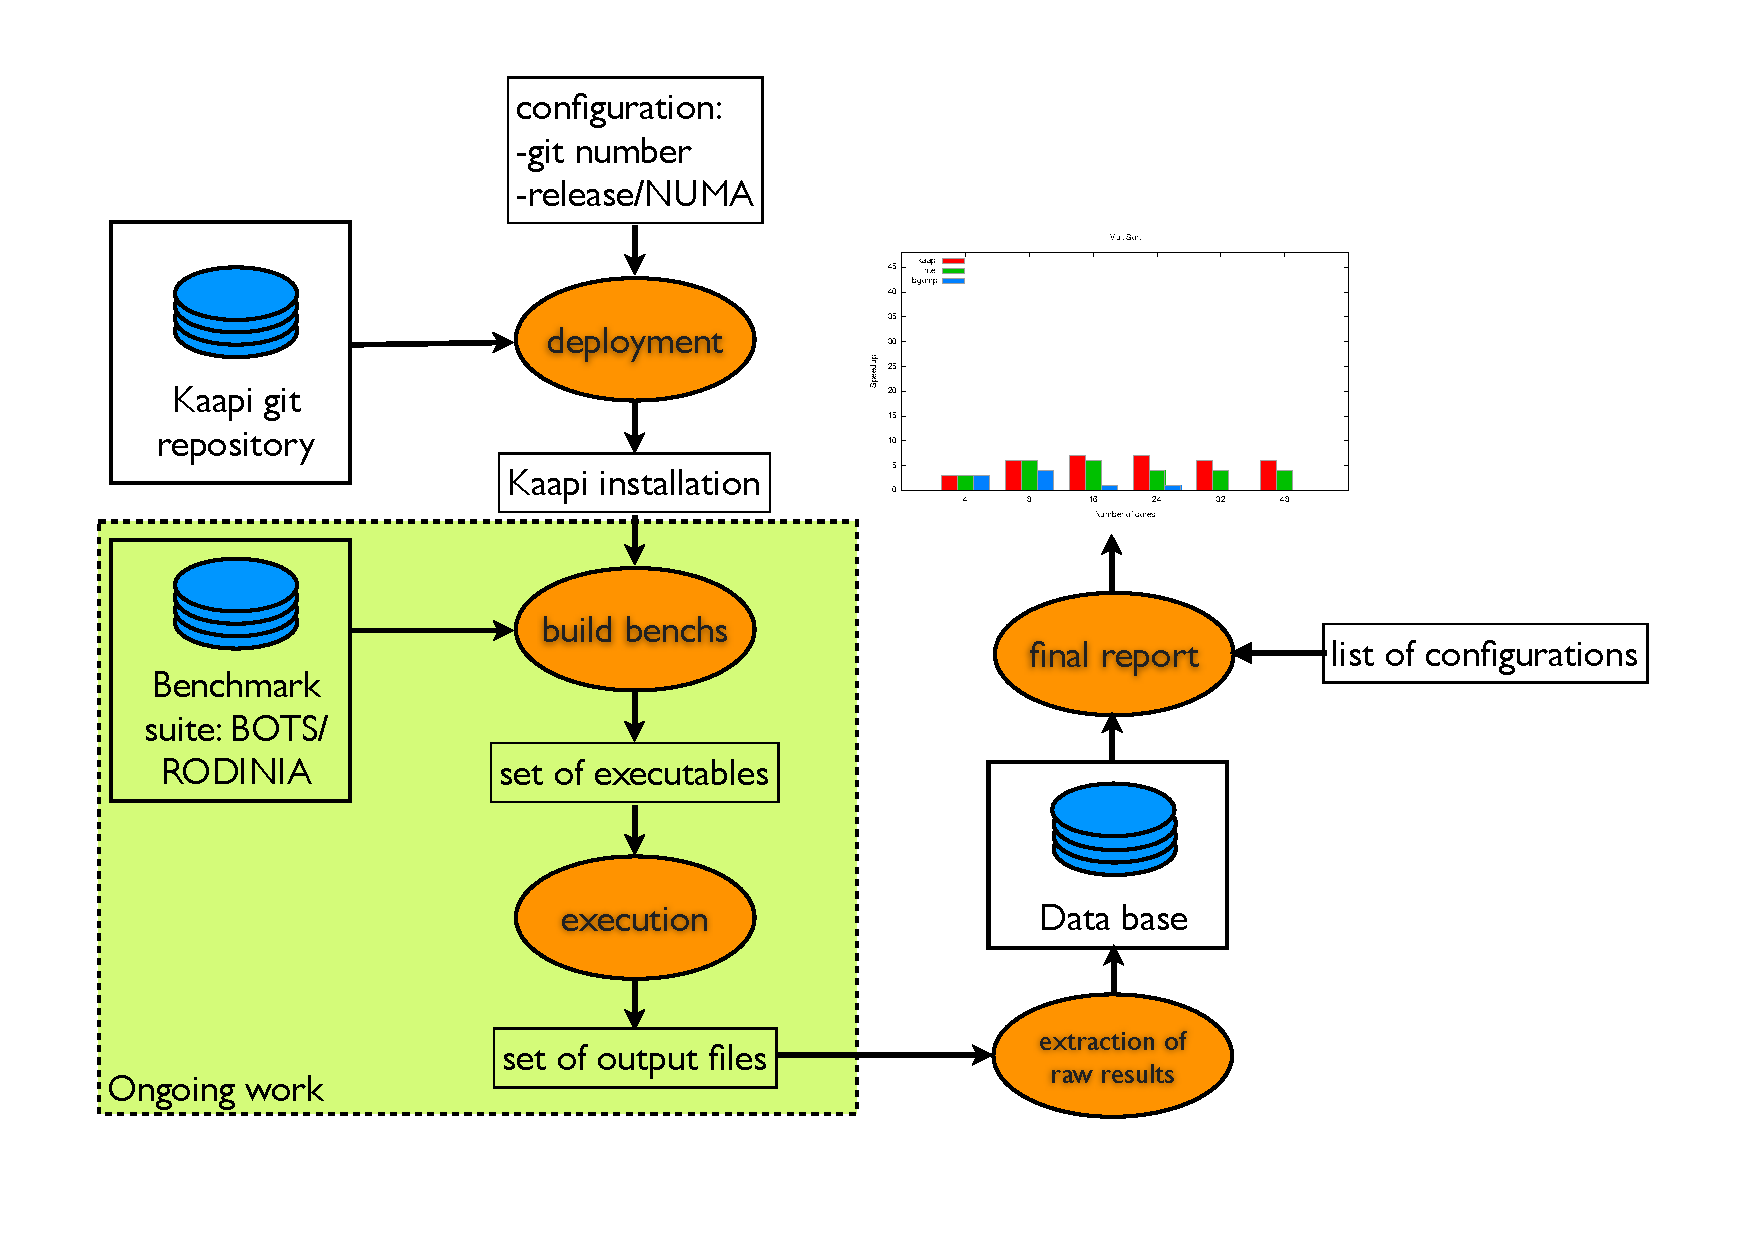
\includegraphics[width=\linewidth]{workflow}
\caption{Global workflow of automatic benchmarking of \kaapi
}
\end{figure}

\bibliographystyle{plain}
\bibliography{rt-kaapi-perf}

\end{document}

%  LocalWords:  runtime
